%% For double-blind review submission, w/o CCS and ACM Reference (max submission space)
%\documentclass[sigplan,review,anonymous]{acmart}\settopmatter{printfolios=true,printccs=false,printacmref=false}
%% For double-blind review submission, w/ CCS and ACM Reference
%\documentclass[sigplan,review,anonymous]{acmart}\settopmatter{printfolios=true}
%% For single-blind review submission, w/o CCS and ACM Reference (max submission space)
%\documentclass[sigplan,review]{acmart}\settopmatter{printfolios=true,printccs=false,printacmref=false}
%% For single-blind review submission, w/ CCS and ACM Reference
%\documentclass[sigplan,review]{acmart}\settopmatter{printfolios=true}
%% For final camera-ready submission, w/ required CCS and ACM Reference
%\documentclass[sigplan]{acmart}\settopmatter{}

\documentclass[sigplan,10pt,review]{acmart}\settopmatter{printfolios=true,printccs=false,printacmref=false}
\usepackage[normalem]{ulem} % double underline
\usepackage{fontspec}
\setmonofont{Cabin}
\setmonofont{Comfortaa}
\setmonofont{Latin Modern Mono Light 10 Bold}
% \setmonofont{FreeMono Bold}
\usepackage{listings}
\definecolor{dkblue}{rgb}{0,0.1,0.5} 
\definecolor{lightblue}{rgb}{0,0.5,0.5} 
\definecolor{dkgreen}{rgb}{0,0.4,0} 
\definecolor{dk2green}{rgb}{0.4,0,0} 
\definecolor{dkviolet}{rgb}{0.6,0,0.8}
%\renewcommand*{\ttdefault}{lmss}
\def\lstlanguagefiles{defManSSR.tex}
\lstset{language=SSR}
\lstset{moredelim=[is][\uwave]{|*}{*|}}
\lstset{moredelim=[is][\uline]{/*}{*/}}
\lstset{moredelim=[is][\dashuline]{|+}{+|}}

\usepackage[english]{babel}
 
%\usepackage{minted}
%\newminted{coq}{fontsize=\footnotesize,escapeinside=\#\#}
 
%% Conference information
%% Supplied to authors by publisher for camera-ready submission;
%% use defaults for review submission.
\acmConference[PL'18]{ACM SIGPLAN Conference on Programming Languages}{January 14--15, 2019}{Lisbon, Protugal}
\acmYear{2019}
\acmISBN{} % \acmISBN{978-x-xxxx-xxxx-x/YY/MM}
\acmDOI{} % \acmDOI{10.1145/nnnnnnn.nnnnnnn}
\startPage{1}

%% Copyright information
%% Supplied to authors (based on authors' rights management selection;
%% see authors.acm.org) by publisher for camera-ready submission;
%% use 'none' for review submission.
\setcopyright{none}
%\setcopyright{acmcopyright}
%\setcopyright{acmlicensed}
%\setcopyright{rightsretained}
%\copyrightyear{2018}           %% If different from \acmYear

%% Bibliography style
\bibliographystyle{ACM-Reference-Format}
%% Citation style
%\citestyle{acmauthoryear}  %% For author/year citations
%\citestyle{acmnumeric}     %% For numeric citations
%\setcitestyle{nosort}      %% With 'acmnumeric', to disable automatic
                            %% sorting of references within a single citation;
                            %% e.g., \cite{Smith99,Carpenter05,Baker12}
                            %% rendered as [14,5,2] rather than [2,5,14].
%\setcitesyle{nocompress}   %% With 'acmnumeric', to disable automatic
                            %% compression of sequential references within a
                            %% single citation;
                            %% e.g., \cite{Baker12,Baker14,Baker16}
                            %% rendered as [2,3,4] rather than [2-4].


%%%%%%%%%%%%%%%%%%%%%%%%%%%%%%%%%%%%%%%%%%%%%%%%%%%%%%%%%%%%%%%%%%%%%%
%% Note: Authors migrating a paper from traditional SIGPLAN
%% proceedings format to PACMPL format must update the
%% '\documentclass' and topmatter commands above; see
%% 'acmart-pacmpl-template.tex'.
%%%%%%%%%%%%%%%%%%%%%%%%%%%%%%%%%%%%%%%%%%%%%%%%%%%%%%%%%%%%%%%%%%%%%%


%% Some recommended packages.
\usepackage{booktabs}   %% For formal tables:
                        %% http://ctan.org/pkg/booktabs
\usepackage{subcaption} %% For complex figures with subfigures/subcaptions
                        %% http://ctan.org/pkg/subcaption


\begin{document}

%% Title information
\title[Deriving proved equality tests, compositionally]{Deriving proved equality tests, compositionally}         %% [Short Title] is optional;
                                        %% when present, will be used in
                                        %% header instead of Full Title.
\titlenote{with title note}             %% \titlenote is optional;
                                        %% can be repeated if necessary;
                                        %% contents suppressed with 'anonymous'
\subtitle{Subtitle}                     %% \subtitle is optional
\subtitlenote{with subtitle note}       %% \subtitlenote is optional;
                                        %% can be repeated if necessary;
                                        %% contents suppressed with 'anonymous'


%% Author information
%% Contents and number of authors suppressed with 'anonymous'.
%% Each author should be introduced by \author, followed by
%% \authornote (optional), \orcid (optional), \affiliation, and
%% \email.
%% An author may have multiple affiliations and/or emails; repeat the
%% appropriate command.
%% Many elements are not rendered, but should be provided for metadata
%% extraction tools.

%% Author with single affiliation.
\author{Enrico Tassi}
\authornote{with author1 note}          %% \authornote is optional;
                                        %% can be repeated if necessary
\orcid{nnnn-nnnn-nnnn-nnnn}             %% \orcid is optional
\affiliation{
  \position{Position1}
  \department{Department1}              %% \department is recommended
  \institution{Institution1}            %% \institution is required
  \streetaddress{Street1 Address1}
  \city{City1}
  \state{State1}
  \postcode{Post-Code1}
  \country{Country1}                    %% \country is recommended
}
\email{Enrico.Tassi@inria.fr}          %% \email is recommended



%% Abstract
%% Note: \begin{abstract}...\end{abstract} environment must come
%% before \maketitle command
\begin{abstract}
We describe a procedure to derive from inductive type declarations
equality tests and their correctness proofs. Programs and proofs
are derived compositionally, reusing code and proofs derived previously.
Finally we provide an implementation for the Coq proof assistant based on the
Elpi extension language.
\end{abstract}


%% 2012 ACM Computing Classification System (CSS) concepts
%% Generate at 'http://dl.acm.org/ccs/ccs.cfm'.
\begin{CCSXML}
<ccs2012>
<concept>
<concept_id>10011007.10011006.10011008</concept_id>
<concept_desc>Software and its engineering~General programming languages</concept_desc>
<concept_significance>500</concept_significance>
</concept>
<concept>
<concept_id>10003456.10003457.10003521.10003525</concept_id>
<concept_desc>Social and professional topics~History of programming languages</concept_desc>
<concept_significance>300</concept_significance>
</concept>
</ccs2012>
\end{CCSXML}

\ccsdesc[500]{Software and its engineering~General programming languages}
\ccsdesc[300]{Social and professional topics~History of programming languages}
%% End of generated code


%% Keywords
%% comma separated list
\keywords{keyword1, keyword2, keyword3}  %% \keywords are mandatory in final camera-ready submission


%% \maketitle
%% Note: \maketitle command must come after title commands, author
%% commands, abstract environment, Computing Classification System
%% environment and commands, and keywords command.
\maketitle

\section{Introduction}

Modern typed programming languages come with the ability of generating
boilerplate code automatically. Typically when a data type is declared
a substantial amount of code is made available to the programmer
at little cost, code such as comparison function, printing function,
generic visitors etc.  The \verb+derive+ directive of Haskell or the
\verb+ppx_deriving+ OCaml preprocessor provide these features for the
respective programming language.

The situation is less than ideal in the Coq proof assistant (others?).
It is capable of generating automatically the recursor of a datatype that
corresponds to induction principle associated to that datatype, such as
lists, but generates a quite disappointing principle when containers are
used to define other types:

\begin{lstlisting}
Inductive rtree A : Type :=
  Leaf (a : A) | Node (l : list (rtree A)).

rtree_ind : forall A (P : rtree A -> Prop),
    (forall a : A, P (Leaf A a)) ->
    (forall l : list (rtree A), P (Node A l)) ->
  forall r : rtree A, P r
\end{lstlisting}

Coq provides a facility to synthesize comparison functions and their proofs
called scheme equality, but it does not support containers.


The need for such tools is made urgent by the structure of
modern formal libraries that are now based on hierarchies of
interfaces. Machinery such as type classes or canonical structures
are used to described the interfaces, and the user is expect to
declare CS or TC instances in order to take advantage of these libraries.
For example first interface one is
required to implement in order to use the theorems in Mathematical
Components library on a type \verb+T+ is the
\verb+eqType+ one, that requires a comparison function on \verb+T+ as
well as a proof of its correctness.

The reason for the status quo is probably caused by a concomitance of
twofold. On one hand the very
expressive type declarations makes it hard to implement a derivation
that fully cover the theory. Even more when the derivation has to be proved
correct. On the other hand meta-programming tools only recently started to appear.

In this paper we focus on the first, base, structure or MC, that is eqType, and
we use the framework for metaprogramming based on elpi developed by the author.

It turns out that generation of eq tests is easy, while their proofs are hard.
One problem is that containers, like lists, come with standard induction principles that are too weak.

eg

and from the fact that termination checking is purely sytnactic, hence 
proofs need to be transparent..

In this paper we describe a derivation proedure where Programs and proofs
are derived compositionally, reusing code and proofs derived previously.

Contributions:
\begin{itemize}
\item a technique to separate, compartimentalize, thee termination checking
	issue by reifying the subterm relation checked by purely syntactic
	means by Coq

\item modular and structured process to derive eqOK. each procedure generates
	terms that can be (re)used separately and

\item actual implementation 
\begin{lstlisting}
Elpi derive rtree.

rtree.eq :
  forall A, (A -> A -> bool) -> rtree A -> rtree A -> bool

rtree.eq.OK :
  forall A (fa : A -> A -> bool) (r : rtree A),
    is_rtree A (axiom A fa) r ->
    axiom (rtree A) (rtree.eq A fa) r

axiom := fun T (eqb : T -> T -> bool) (x : T) =>
     forall y : T, reflect (x = y) (eqb x y)
\end{lstlisting}
\end{itemize}

Strucure.

\section{The problem: eq proofs meets syntactic termination checking}

induction principles are not primitive, but encoded as fix + match, hence one
can still prove

fix f => ... eqlistok f ..

This, in order to be "type checked" requires the system to inspect the
full proof of eqlistok since The check is syntactic.

What the syntactic check tries to capture is the following relation:
Is a subterm of the same type.

this is 

\section{decorrelating terms and types: unary parametricity by examples}

\begin{lstlisting}
Inductive is_nat : nat -> Type :=
| is_O : is_nat 0
| is_S n (pn : is_nat n) : is_nat (S n)
\end{lstlisting}

for containers

\begin{lstlisting}
Inductive is_list A (PA : A -> Type) : list A -> Type :=
| is_nil : is_list A PA nil
| is_cons a (pa : PA a) l (pl : is_list A PA l) :
    is_list A PA (a :: l)
\end{lstlisting}

An instance of \cite{keller:hal-00730913}

\subsection{(truncated?) induction principle from tR}

\begin{lstlisting}
list_ind :
  forall A (P : list A -> Prop),
    P nil ->
    (forall a l, P l -> P (a :: l)) ->
  forall l : list A, P l

list.induction.principle :
  forall A /*(PA : A -> Type)*/ (P : list A -> Type),
    P nil ->
    (forall a /*(pa : PA a)*/ l, P l -> P (a :: l)) ->
  forall l, /*is_list A PA l*/ -> P l

is_list_ind :
  forall A (PA : A -> Type) (P : forall l, |*is_list A PA l ->*| Prop),
    P nil |*(is_list.nil A PA)*| ->
    (forall a (pa : PA a) l |*(pl : is_list A PA l)*|, P l |*pl*| ->
        P (a :: l) |* (is_cons A PA a pa l pl)*|) ->
  forall l (pl : is_list A PA s), P l |*pl*| *)

\end{lstlisting}


\subsection{compartmentalizing of the syntactic check}

\begin{lstlisting}
is_rtreeP : forall A (PA : A -> Type),
  (forall x, PA x) -> forall t, is_rtree A PA t
\end{lstlisting}

this is needed to close the thing we recall here

\begin{lstlisting}
rtree.eq.OK : forall A (fa : A -> A -> bool) (s1 : rtree A),
  is_rtree A (axiom A fa) s1 ->
  axiom (rtree A) (rtree.eq A fa) s1

nat.eq.OK : forall n, axiom nat nat.eq n
\end{lstlisting}


\section{structure} %%%%%%%%%%%%%%%%%%%%%%%%%%%%%%%%%%%%%%%%%%%%%%%%%%%%%%%%

\begin{figure*}
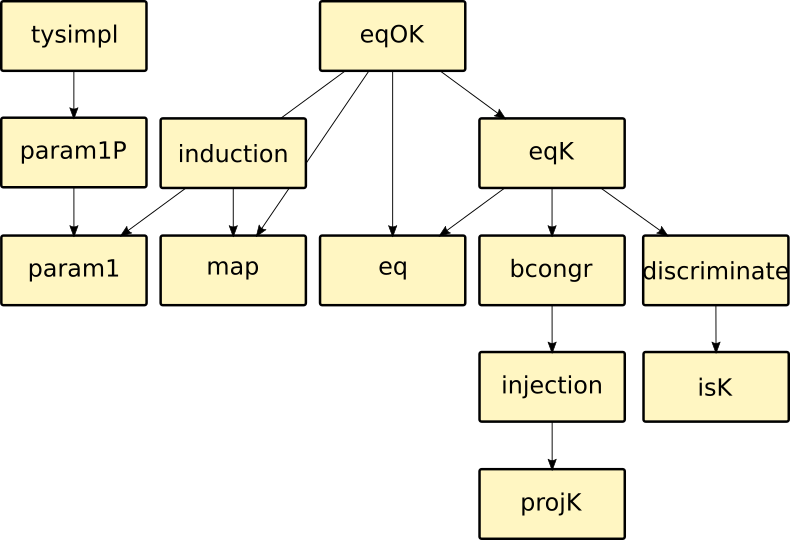
\includegraphics[width=0.6\textwidth]{derive.png}
\end{figure*}

structure of the proof



\subsection{param1 and param1P} %%%%%%%%%%%%%%%%%%%%%%%%%%%%%%%%%%%%%%%%%%%


\begin{lstlisting}
Inductive is_rtree A (PA : A -> Type) : rtree A -> Type :=
| Leaf a (pa : PA a) : is_rtree A PA (Leaf A a)
| Node l (pl : is_list (is_rtree A) (is_rtree A PA) l) :
    is_rtree A PA (Node A l)
	   
is_rtreeP : forall A (PA : A -> Type),
  (forall x, PA x) -> forall t, is_rtree A PA t
\end{lstlisting}


\subsection{map} %%%%%%%%%%%%%%%%%%%%%%%%%%%%%%%%%%%%%%%%%%%%%%%%%%%%%%%%%%%

map for containers is what one expects.

\begin{lstlisting}
rtree.map : forall A1 A2, (A1 -> A2) -> rtree A1 -> rtree A2
\end{lstlisting}

indexes are not mapped, and hence the variables
used in their types are not mapped

predicates are made implications

\marginpar{fails on rtree}

\begin{lstlisting}
is_list.map : forall A PA PB l,
  (forall x, PA x -> PB x) -> is_list A PA l -> is_list A PB l
\end{lstlisting}

functoriality

\subsection{induction} %%%%%%%%%%%%%%%%%%%%%%%%%%%%%%%%%%%%%%%%%%%%%%%%%%%%%%

take tR and do the obvious induction for it, then truncate P.

\subsection{isK and discriminate} %%%%%%%%%%%%%%%%%%%%%%%%%%%%%%%%%%%%%%%%%%%%

\begin{lstlisting}
rtree.is.Node : forall A : Type, rtree A -> bool
rtree.is.Leaf : forall A : Type, rtree A -> bool
eq_f : forall T1 T2 (f : T1 -> T2) a b, a = b -> f a = f b.
bool_discr : true = false -> forall T : Type, T.
\end{lstlisting}

\subsection{projK and injection} %%%%%%%%%%%%%%%%%%%%%%%%%%%%%%%%%%%%%%%%%%%%%

\begin{lstlisting}
list.injection.cons1 : forall A, A -> list A -> list A -> A
list.injection.cons2 : forall A, A -> list A -> list A -> list A
\end{lstlisting}
to be used in conjunction with \lstinline+eq_f+ in case one has

\begin{lstlisting}
H : cons x xs = cons y ys
eqf H (list.injection.cons2 A x xs) : xs = ys
\end{lstlisting}

The type is so that the function can be total and given the use
case one can always pass the arguments of the constructor on the
LHS of H.

\begin{lstlisting}
list.injection.cons1 = 
  fun (A : Type) (default1 : A) (default2 : list A) (l : list A) =>
    match l with
    | nil => default1
    | x :: _ => x
    end
\end{lstlisting}

\subsection{bcongr} %%%%%%%%%%%%%%%%%%%%%%%%%%%%%%%%%%%%%%%%%%%%%%%%%%%%%%%

\begin{lstlisting}
list.eq.bcongr.cons : forall A,
    forall (x y : A) b, reflect (x = y) b ->
    forall (xs ys : list A) c, reflect (xs = ys) c ->
  reflect (x :: xs = y :: ys) (b && c)

rtree.eq.bcongr.Leaf : forall A (x y : A) b,
  reflect (x = y) b -> reflect (Leaf A x = Leaf A y) b
\end{lstlisting}

\subsection{eq} %%%%%%%%%%%%%%%%%%%%%%%%%%%%%%%%%%%%%%%%%%%%%%%%%%%%%%%%%%

\begin{lstlisting}
rtree.eq = 
  fun (A : Type) (eqA : A -> A -> bool) =>
    fix rec (t1 t2 : rtree A) {struct t1} : bool :=
    match t1, t2 with
    | Leaf a, Leaf b  => eqA a b
    | Node l, Node s => list.eq (rtree A) rec l s
    | _, _ => false
    end
\end{lstlisting}

\subsection{eqK and eqOK} %%%%%%%%%%%%%%%%%%%%%%%%%%%%%%%%%%%%%%%%%%%%%%%%

\begin{lstlisting}
rtree.eq.axiom.Node : forall A (f : A -> A -> bool) l,
    axiom (list (rtree A)) (list.eq (rtree A) (rtree.eq A f)) l ->
  axiom (rtree A) (rtree.eq A f) (Node A l)
\end{lstlisting}

\begin{lstlisting}
list.eq.correct : forall A (fa : A -> A -> bool) l,
    is_list A (axiom A fa) l ->
  axiom (list A) (list.eq A fa) l
       
rtree.eq.correct = fun A (fa : A -> A -> bool) =>
  rtree.induction.principle A (axiom A fa)
    (axiom (rtree A) (rtree.eq A fa)) (* P *)
    (rtree.eq.axiom.Leaf A fa)
    (fun l (Pl : is_list (rtree a)
                   (axiom (rtree a) (rtree.eq a fa)) l) =>
      rtree.eq.axiom.Node A fa l
        (list.eq.correct (rtree a) (rtree.eq a fa) l Pl))
: forall (A : Type) (fa : A -> A -> bool) (t : rtree A),
    is_rtree A (axiom A fa) t ->
    axiom (rtree A) (rtree.eq A fa) t
\end{lstlisting}

\subsection{tysimpl} %%%%%%%%%%%%%%%%%%%%%%%%%%%%%%%%%%%%%%%%%%%%%%%%%%%%%

\begin{lstlisting}
nat.induction.principle : forall P : nat -> Type,
    P 0 -> (forall p : nat, P p -> P (S p)) ->
  forall n, is_nat n -> P n

nat.induction = fun P HO HS n =>
    nat.induction.principle P HO HS n (is_natP n)
: forall P : nat -> Type,
    P 0 -> (forall p, P p -> P (S p)) ->
  forall n, P n
\end{lstlisting}


%%%%%%%%%%%%%%%%%%%%%%%%%%%%%%%%%%%%%%%%%%%%%%%%%%%%%%%%%%%%%%%%%%%%%%%%%%%
\section{implementation} %%%%%%%%%%%%%%%%%%%%%%%%%%%%%%%%%%%%%%%%%%%%%%%%%%

Coq-elpi links a PL based on lambda Prolog and CHR.
The latter fragment plays no role in this paper.
lambda Prolog uses HOAS to describe Coq terms.
logic programming has an obvious way of describing the db of
knowledge, for example in eq-db.

api do provide access rw to the env

\subsection{incompleteness and user intervention} %%%%%%%%%%%%%%%%%%%%%%%%%

mut ind no supported by elpi. while they make code longer we don't see
which additional difficulty they could bring.

univ polymorphism not supported by elpi. no additional complexity.

eqtype is prerequisite for indexes decidable. the algorithm
consists in packing inductive { .. } for contextual reasoning
and finally projecting. As of today it is not fully automatized, but
the chain can be used by manually providing the bloks that are missing.

%%%%%%%%%%%%%%%%%%%%%%%%%%%%%%%%%%%%%%%%%%%%%%%%%%%%%%%%%%%%%%%%%%%%%%%%%%
\section{related work} %%%%%%%%%%%%%%%%%%%%%%%%%%%%%%%%%%%%%%%%%%%%%%%%%%%

Coq: scheme equality (no containers in ty of constructors),
decide equality works but one has to do the fix by hand + inlines everything
+ termination check.

Lean: rec/ind + discr
Agda: no.
Haskell: TODO.
OCaml: ppx deriving.
McBride: polytypes. Isabelle?

%%%%%%%%%%%%%%%%%%%%%%%%%%%%%%%%%%%%%%%%%%%%%%%%%%%%%%%%%%%%%%%%%%%%%%%%%%%
\section{conclusion} %%%%%%%%%%%%%%%%%%%%%%%%%%%%%%%%%%%%%%%%%%%%%%%%%%%%%%

not done before because of the lack of a platform that makes experimentation
easy.

some bricks are reusable, eg in tactics.

call for size types.

\begin{acks}
We thank Maxime Denes and Cyril Cohen for many discussions shedding light
on the subject; Cyril Cohen for the code implementing the parametricity
translation in Elpi; Luc Chabassier for working on an early prototype of
Elpi on the synthesis of equality tests, an experiment that convinced
the author it was actually doable.
\end{acks}


%% Bibliography
\bibliography{bibfile}


%% Appendix
\appendix
\section{Appendix}

Text of appendix \ldots

\end{document}
